\chapter{Alur Implementasi Penegakan Otoritas pada Server PRE}
\label{lampiran:alur-implementasi-penegakan-otoritas-pre}

Alur penegakan otoritas pada \textit{Server} PRE diilustrasikan dalam dua buah flow diagram yang saling berkelanjutan, sebagaimana ditunjukkan pada Gambar \ref{fig:alur-penegakan-otoritas-pre-a} dan \ref{fig:alur-penegakan-otoritas-pre-b}. Gambar \ref{fig:legenda-flowdiag-penegakan-otoritas-pre} memuat legenda bentuk pada \textit{Flow Diagram}.

\begin{figure}[ht]
	\centering
	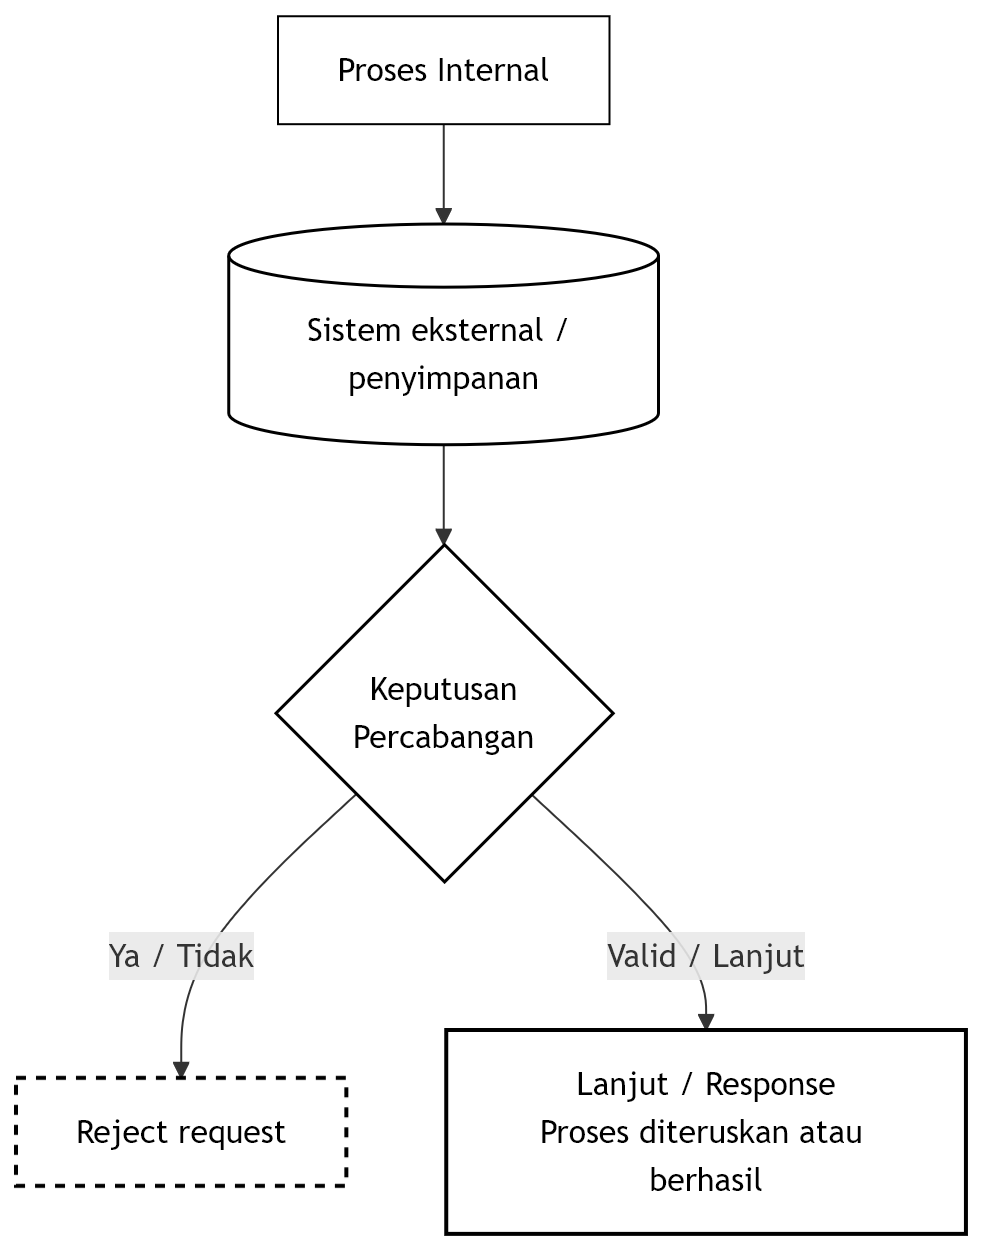
\includegraphics[width=0.65\textwidth,keepaspectratio]{resources/appendix/legenda flowdiag.png}
	\caption{Legenda bentuk pada \textit{Flow Diagram}}
	\label{fig:legenda-flowdiag-penegakan-otoritas-pre}
\end{figure}

\begin{figure}[ht]
	\centering
	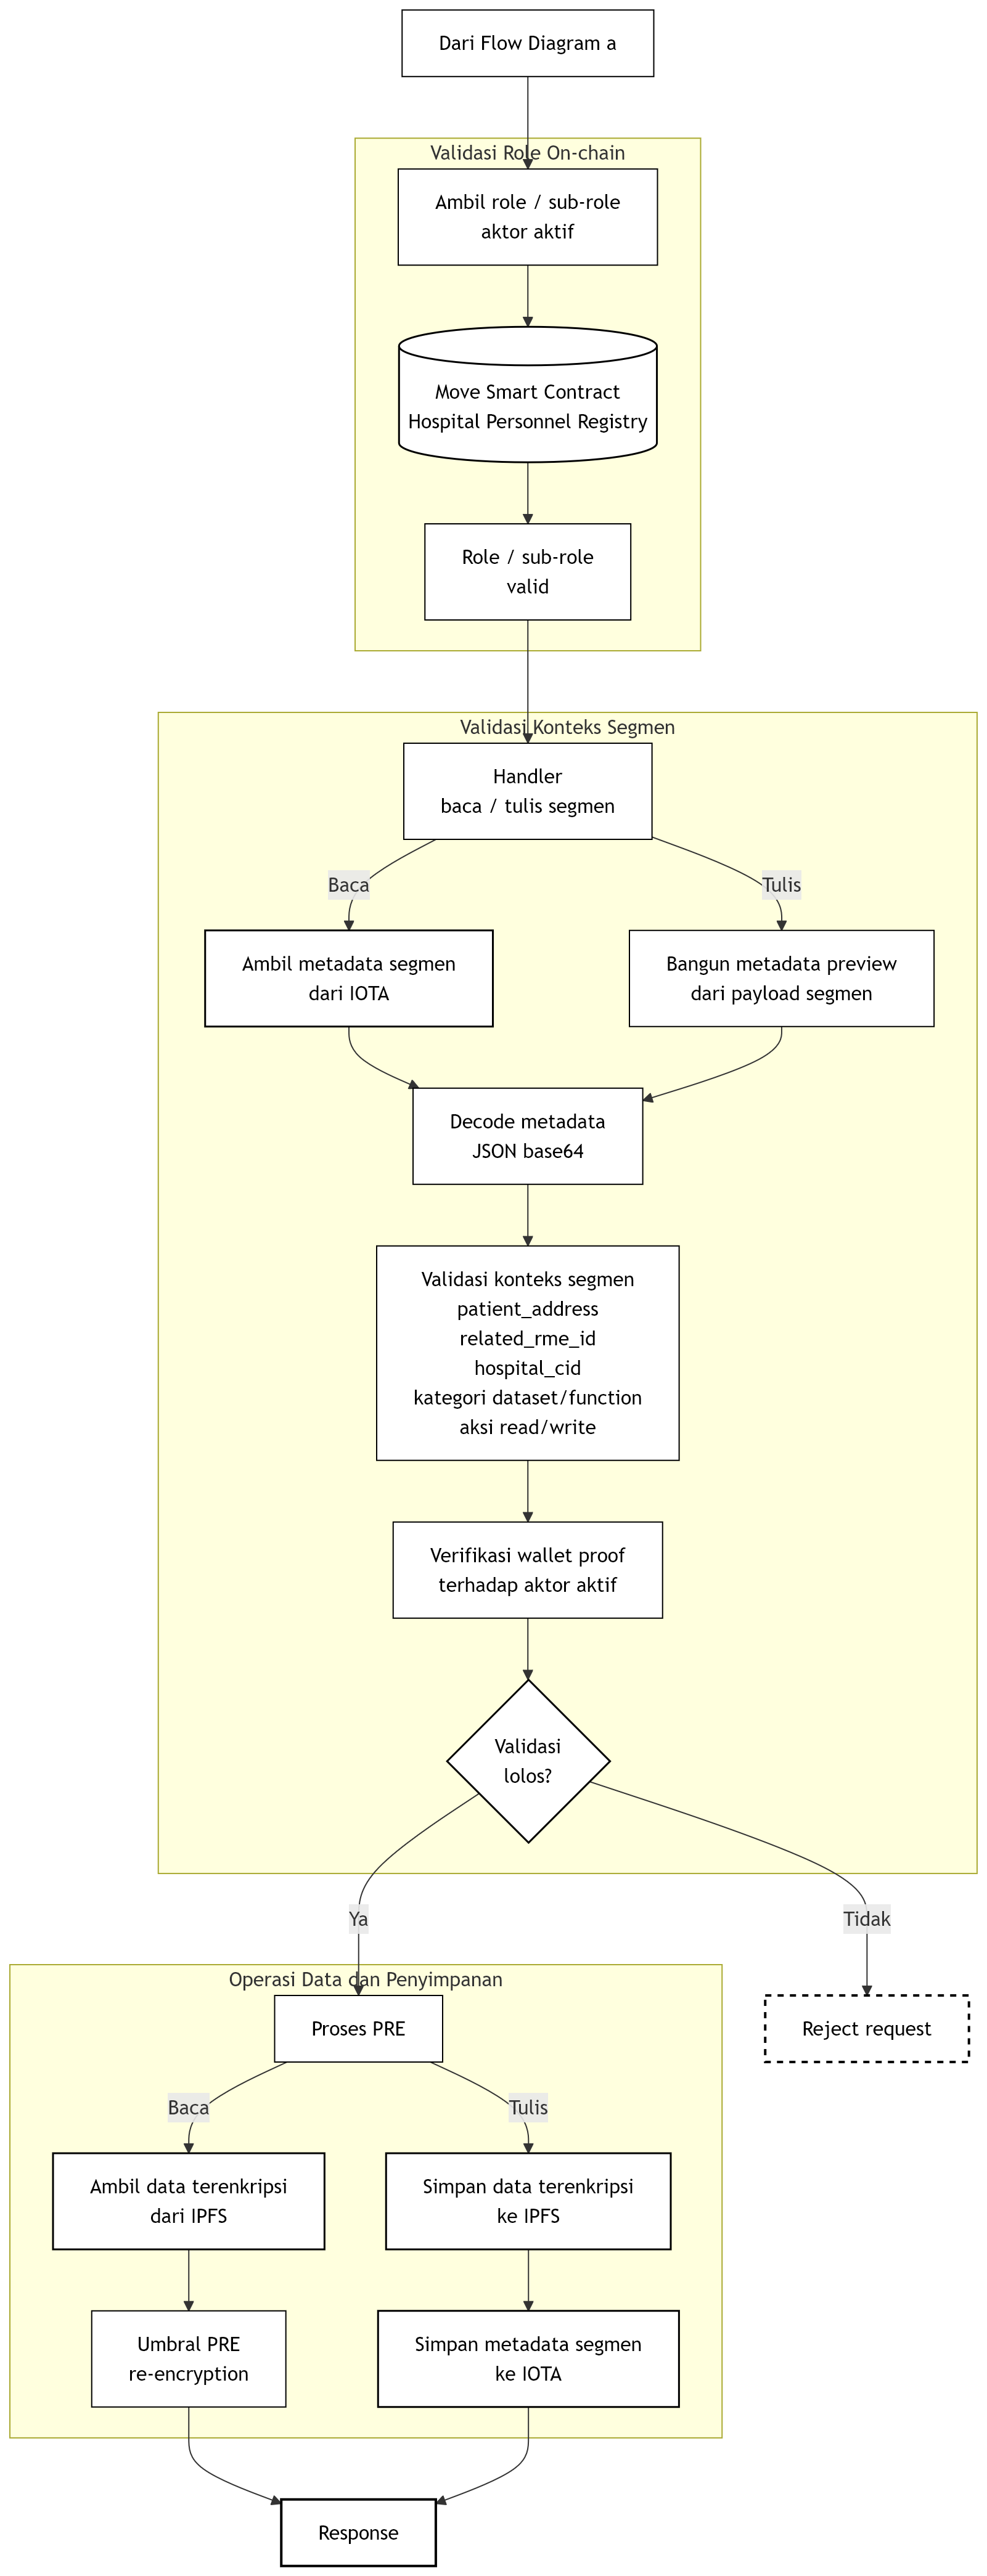
\includegraphics[height=0.8\textheight,keepaspectratio]{resources/appendix/flowdiag-penegakan otorisasi a.png}
	\caption{Alur implementasi penegakan otoritas pada \textit{Server} PRE bagian autentikasi token, \textit{effective capability}, \textit{delegation chain}, dan revokasi}
	\label{fig:alur-penegakan-otoritas-pre-a}
\end{figure}

\begin{figure}[ht]
	\centering
	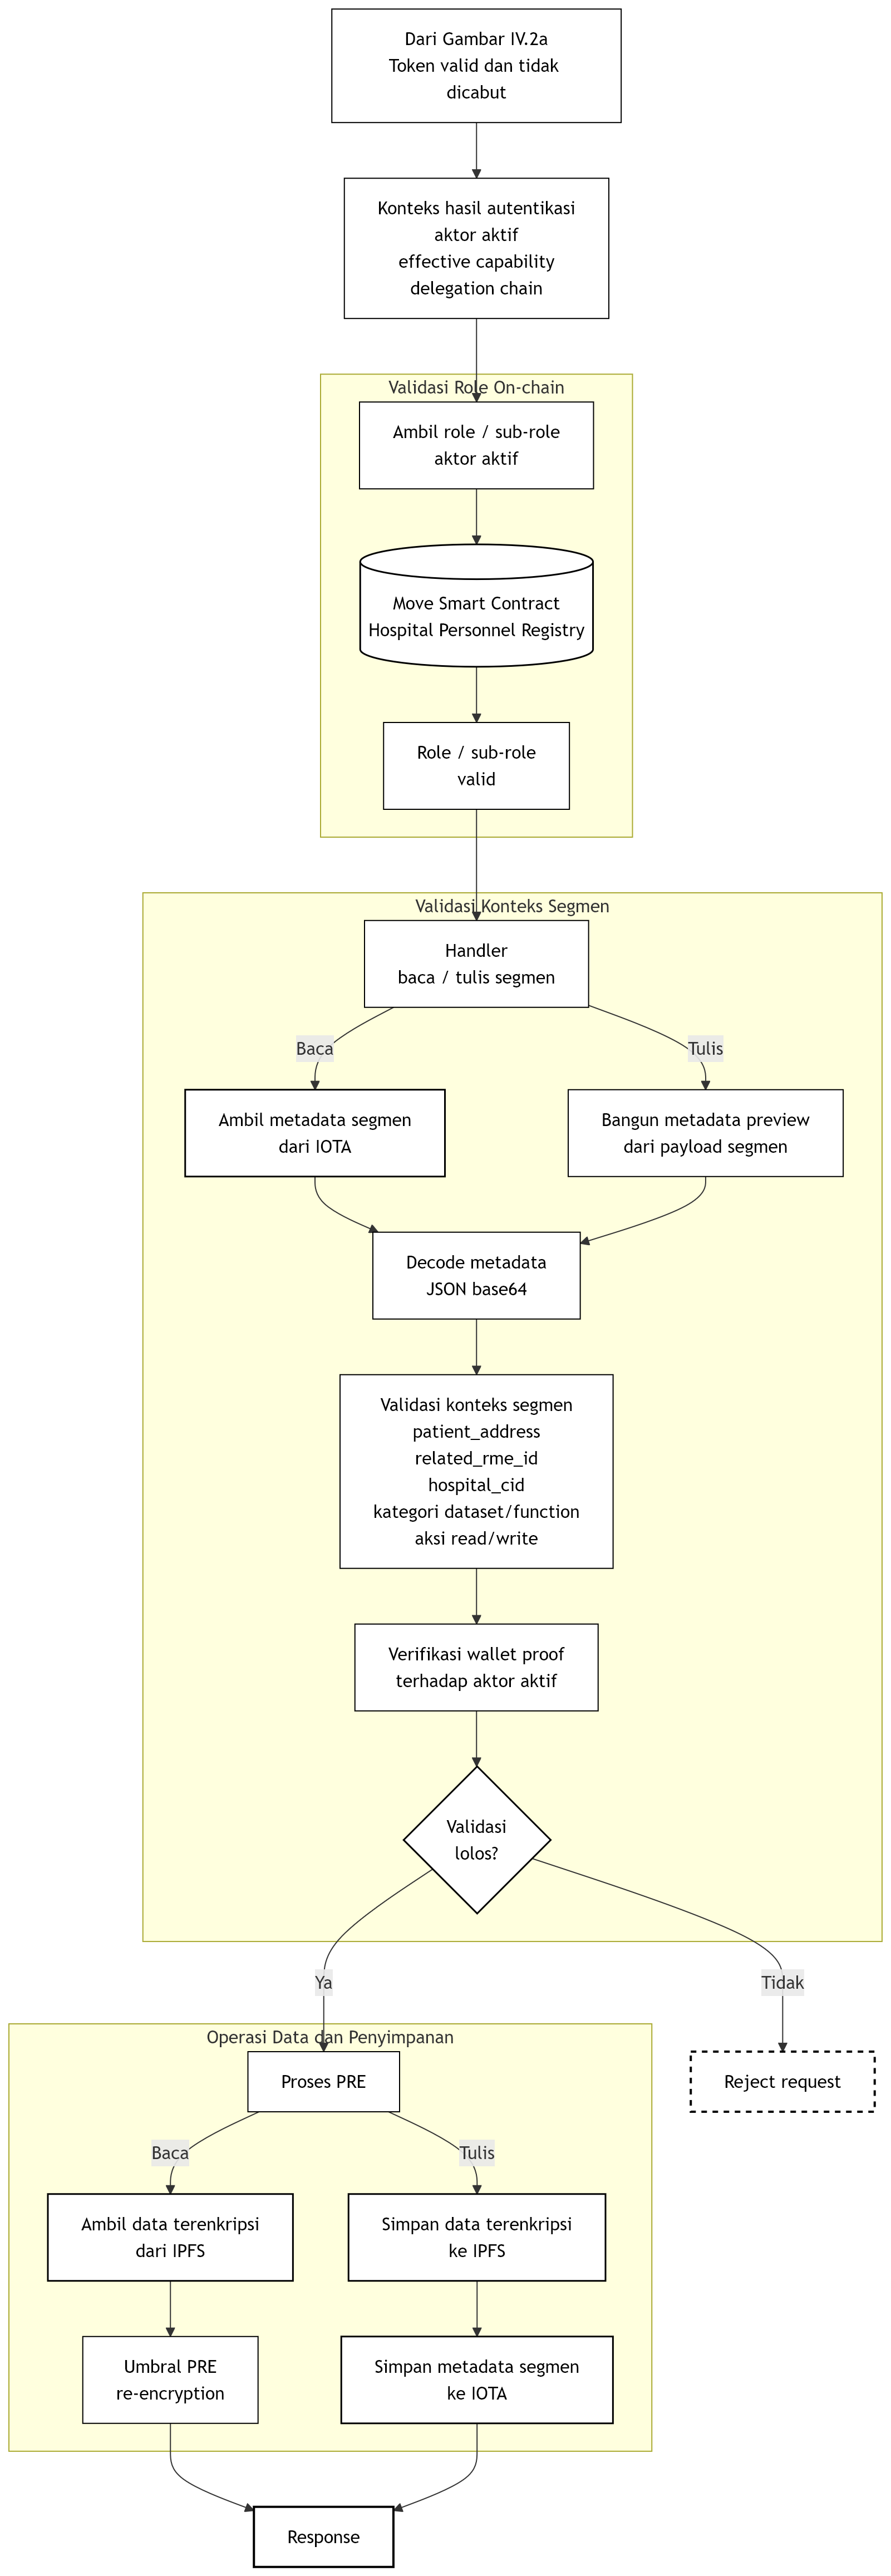
\includegraphics[height=0.8\textheight,keepaspectratio]{resources/appendix/flowdiag-penegakan otorisasi b.png}
	\caption{Alur implementasi penegakan otoritas pada \textit{Server} PRE bagian validasi \textit{role} dan \textit{subrole}, validasi segmen, \textit{wallet proof}, serta eksekusi PRE, IPFS, dan IOTA}
	\label{fig:alur-penegakan-otoritas-pre-b}
\end{figure}
